% This LaTeX was auto-generated from MATLAB code.
% To make changes, update the MATLAB code and export to LaTeX again.

\documentclass{article}

\usepackage[utf8]{inputenc}
\usepackage[T1]{fontenc}
\usepackage{lmodern}
\usepackage{graphicx}
\usepackage{color}
\usepackage{hyperref}
\usepackage{amsmath}
\usepackage{amsfonts}
\usepackage{epstopdf}
\usepackage[table]{xcolor}
\usepackage{matlab}

\sloppy
\epstopdfsetup{outdir=./}
\graphicspath{ {./perceptron_example_images/} }

\begin{document}

\matlabtitle{Perceptron Example}

\begin{matlabcode}
rng(5)
X = rand([100,1]);
y = 2*(double(X>0.5)-0.5*ones(size(X)));

f=gscatter(X,zeros(size(X)),y,'br','o');
hold on
ylim([-0.1,0.1])
hold off
\end{matlabcode}
\begin{center}
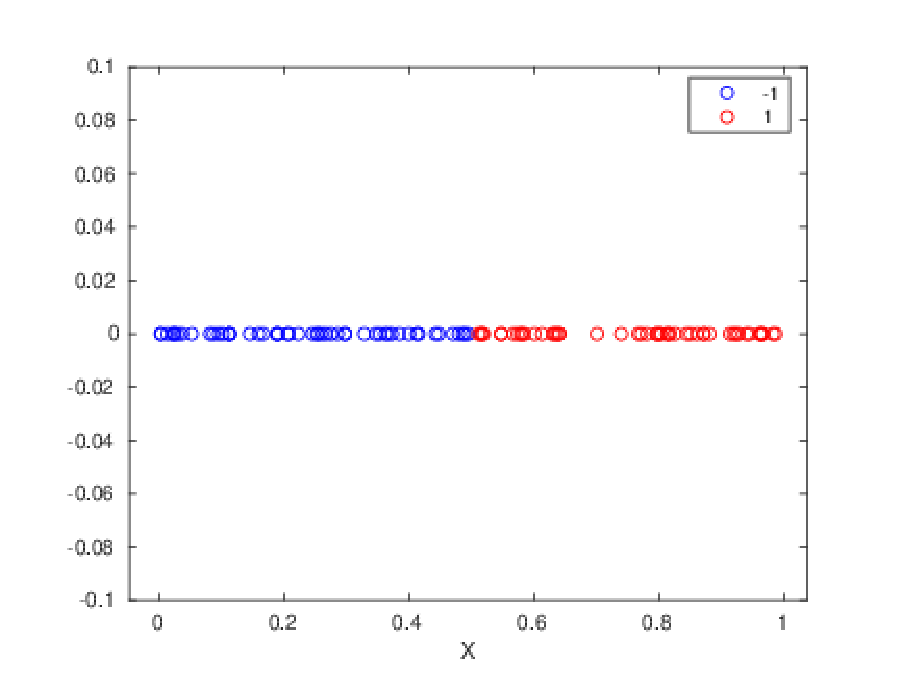
\includegraphics[width=\maxwidth{56.69844455594581em}]{figure_0.eps}
\end{center}



\vspace{1em}
\begin{par}
\begin{flushleft}
Now, let's manually use our perceptron:
\end{flushleft}
\end{par}

\begin{matlabcode}
W = [-0.5; 1]
\end{matlabcode}
\begin{matlaboutput}
W = 2x1    
   -0.5000
    1.0000

\end{matlaboutput}
\begin{matlabcode}

% Add the bias
X_bias = [ones(size(X)) X];

pred = zeros(size(X));

for i=1:length(X)
    x = X_bias(i,:)';
    S = state(x,W);
    pred(i) = my_sign(S);
end

f2=gscatter(X,zeros(size(X)),pred,'br','o');
hold on
ylim([-0.1,0.1])
hold off
\end{matlabcode}
\begin{center}
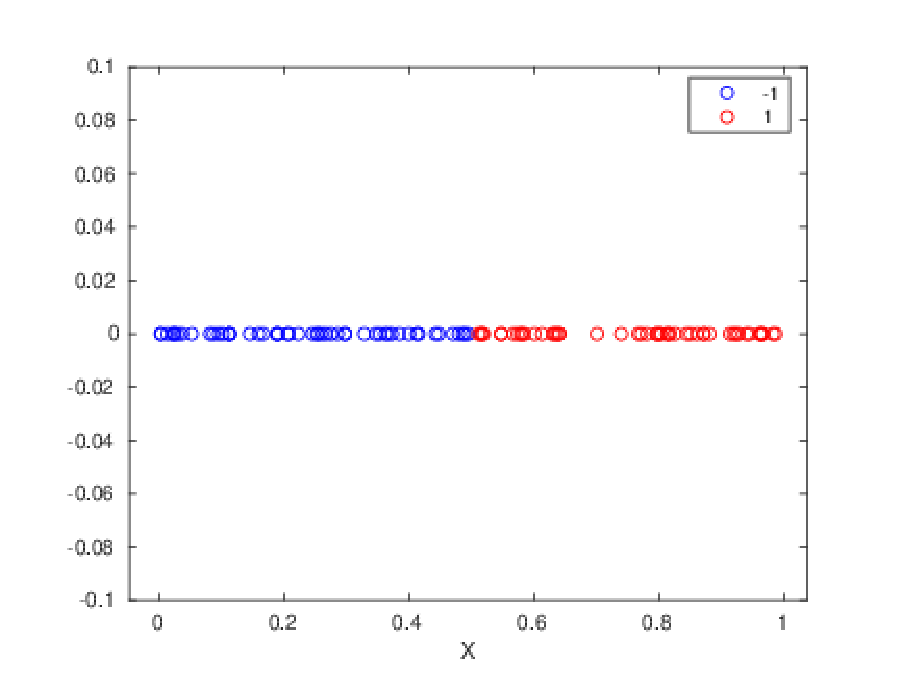
\includegraphics[width=\maxwidth{56.69844455594581em}]{figure_1.eps}
\end{center}


\begin{par}
\begin{flushleft}
It classified perfectly! Now let's train the algorithm:
\end{flushleft}
\end{par}

\begin{matlabcode}
% Add the bias
X_bias = [ones(size(X)) X];

% Train the model
W2 = train(X_bias,y,0.1,10)
\end{matlabcode}
\begin{matlaboutput}
W2 = 2x1    
   -0.1000
    0.2013

\end{matlaboutput}
\begin{matlabcode}

pred2 = zeros(size(X_bias));

for i=1:length(X)
    x = X_bias(i,:)';
    S = state(x,W2);
    pred2(i) = my_sign(S);
end

f3=gscatter(X,zeros(size(X)),pred2,'br','o');
hold on
ylim([-0.1,0.1])
hold off
\end{matlabcode}
\begin{center}
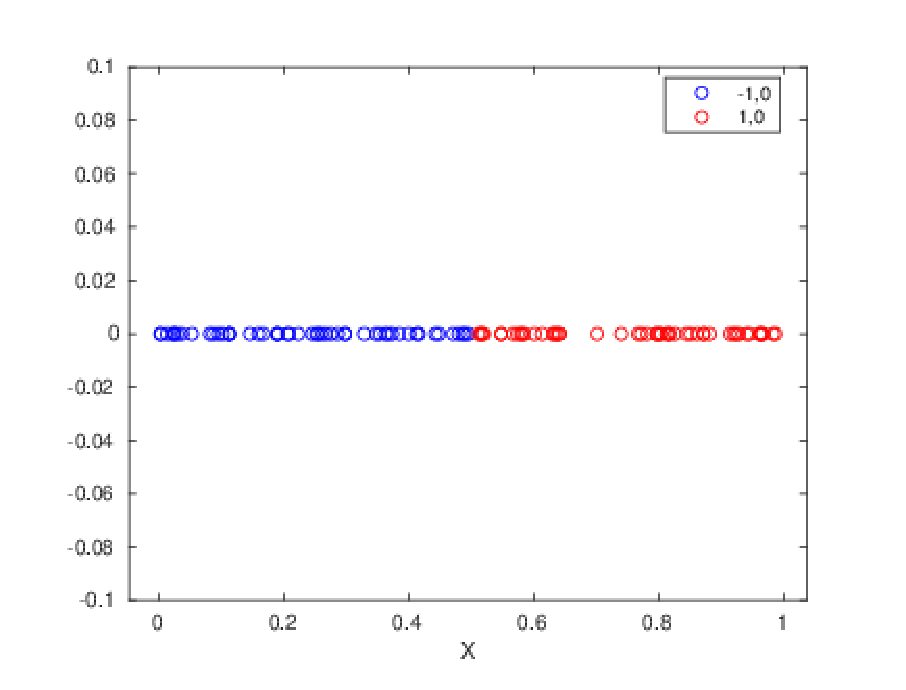
\includegraphics[width=\maxwidth{56.69844455594581em}]{figure_2.eps}
\end{center}

\begin{par}
\begin{flushleft}
This is quite interesting... it found different weights, but it classified eveything well. This must break somewhere. Let's try to determine where:
\end{flushleft}
\end{par}


\begin{matlabcode}
X = 0.45:0.001:0.55;
X = X';
y = 2*(double(X>0.5)-0.5*ones(size(X)));

X_bias = [ones(size(X)) X];

pred3 = zeros(size(X));

for i=1:length(X)
    x = X_bias(i,:)';
    S = state(x,W2);
    pred3(i) = my_sign(S);
end

f4=gscatter(X_bias,zeros(size(X)),pred3==y,'br','o');
hold on
ylim([-0.1,0.1])
xlim([0.45,0.55])
hold off
\end{matlabcode}
\begin{center}
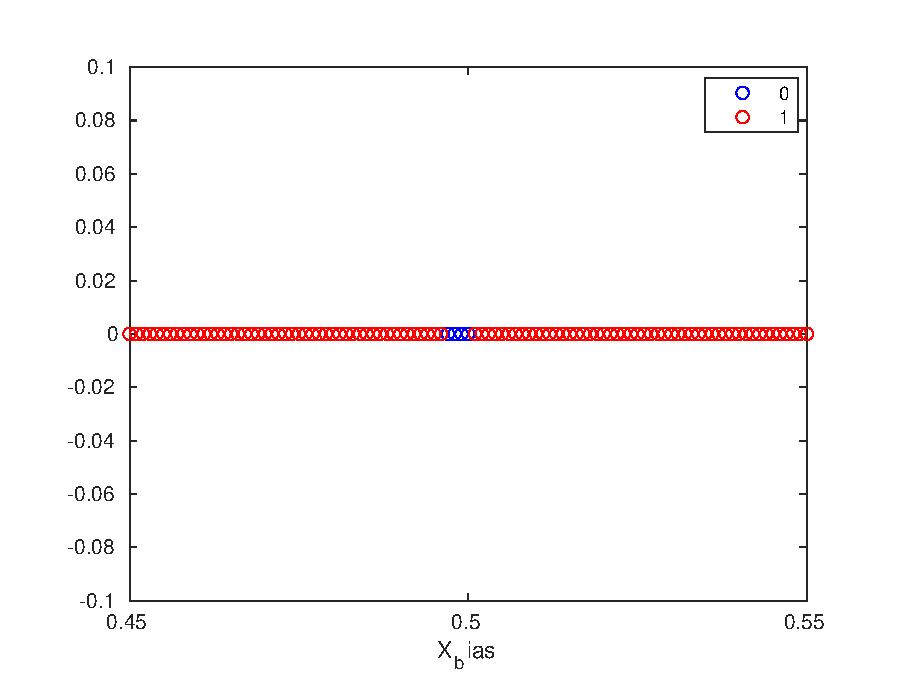
\includegraphics[width=\maxwidth{56.69844455594581em}]{figure_3.eps}
\end{center}
\begin{matlabcode}

y(pred3~=y)
\end{matlabcode}
\begin{matlaboutput}
ans = 4x1    
    -1
    -1
    -1
    -1

\end{matlaboutput}

\begin{par}
\begin{flushleft}
This means that our model is actually setting the bound a little bit before 0.5 (as can be seen in the graph). This should be improved by increasing the size of X.
\end{flushleft}
\end{par}


\begin{matlabcode}
function S = state(X, W)
    S = W'*X;
end

function pred = my_sign(S)
    if S > 0
        pred = 1;
    else
        pred = -1;
    end
end

function W = train(X, y, lr, epochs)
    [~, d] = size(X);
    W = zeros(d, 1);
    for epoch = 1:epochs
        for i = 1:length(X)
            x = X(i,:)';
            pred = my_sign(state(x, W));
            if pred ~= y(i)
                W = W + lr*x*y(i);
            end
        end
    end
end

\end{matlabcode}

\end{document}
